\chapter{Task 3}
\section{UseCase View}
\begin{figure}[hbt]
  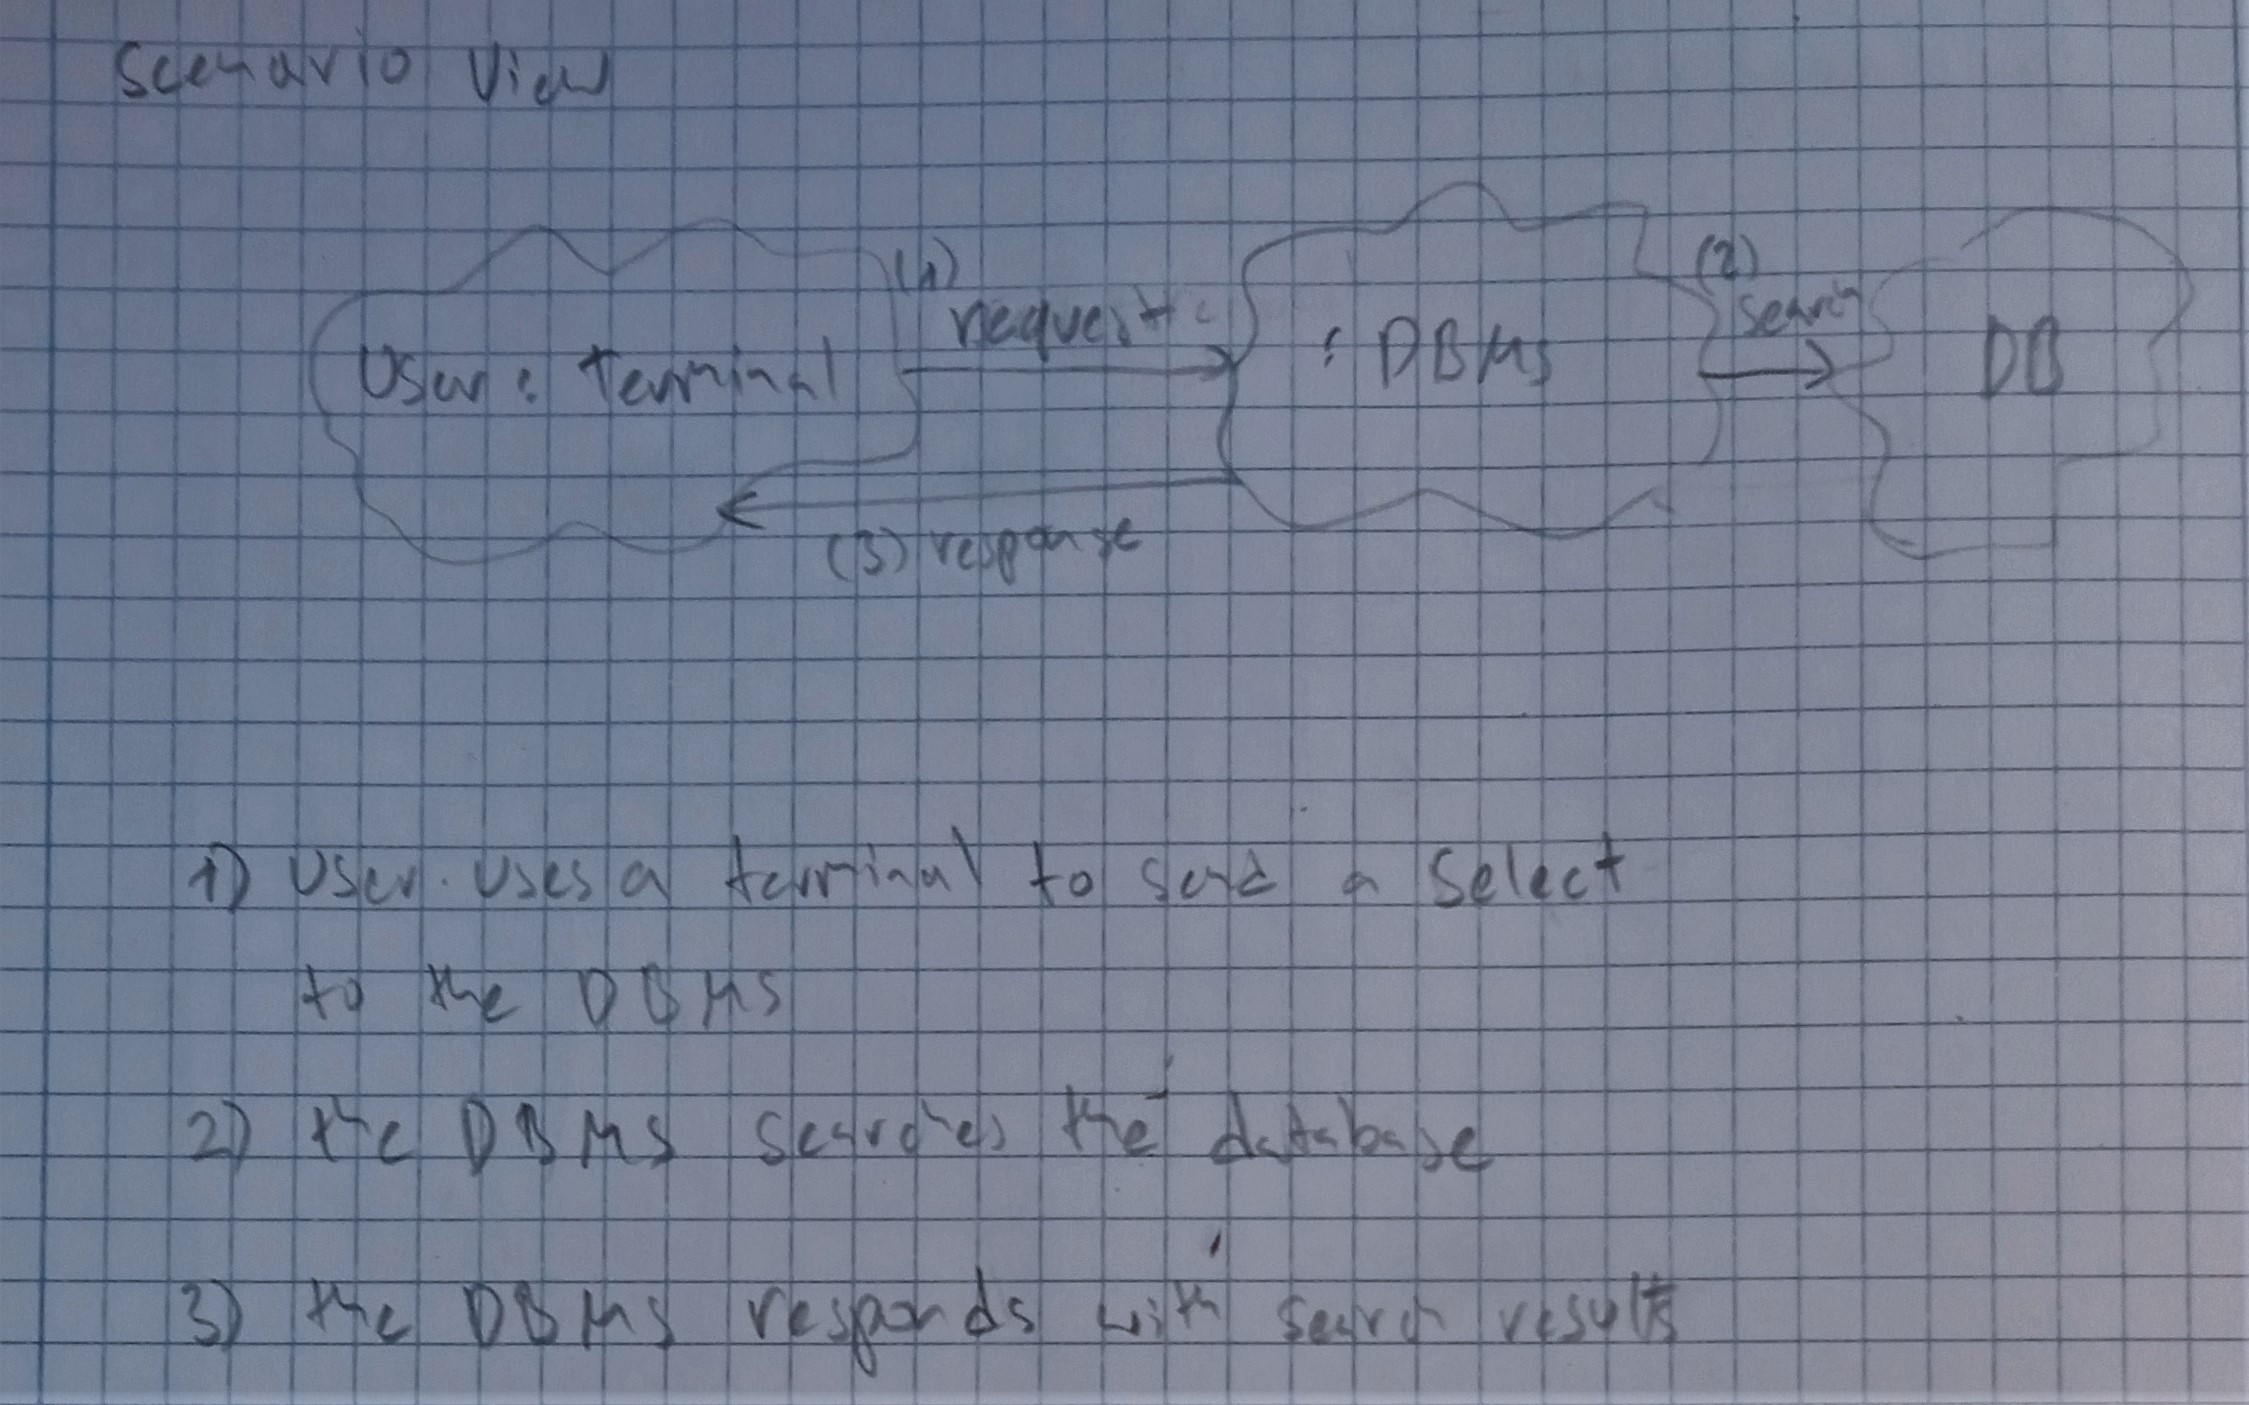
\includegraphics[width=\textwidth]{Immagini/IMG_20230604_171749.jpg}
  \caption{UseCase View}
\end{figure}


\begin{figure}[hbt]
\section{Logical View}
  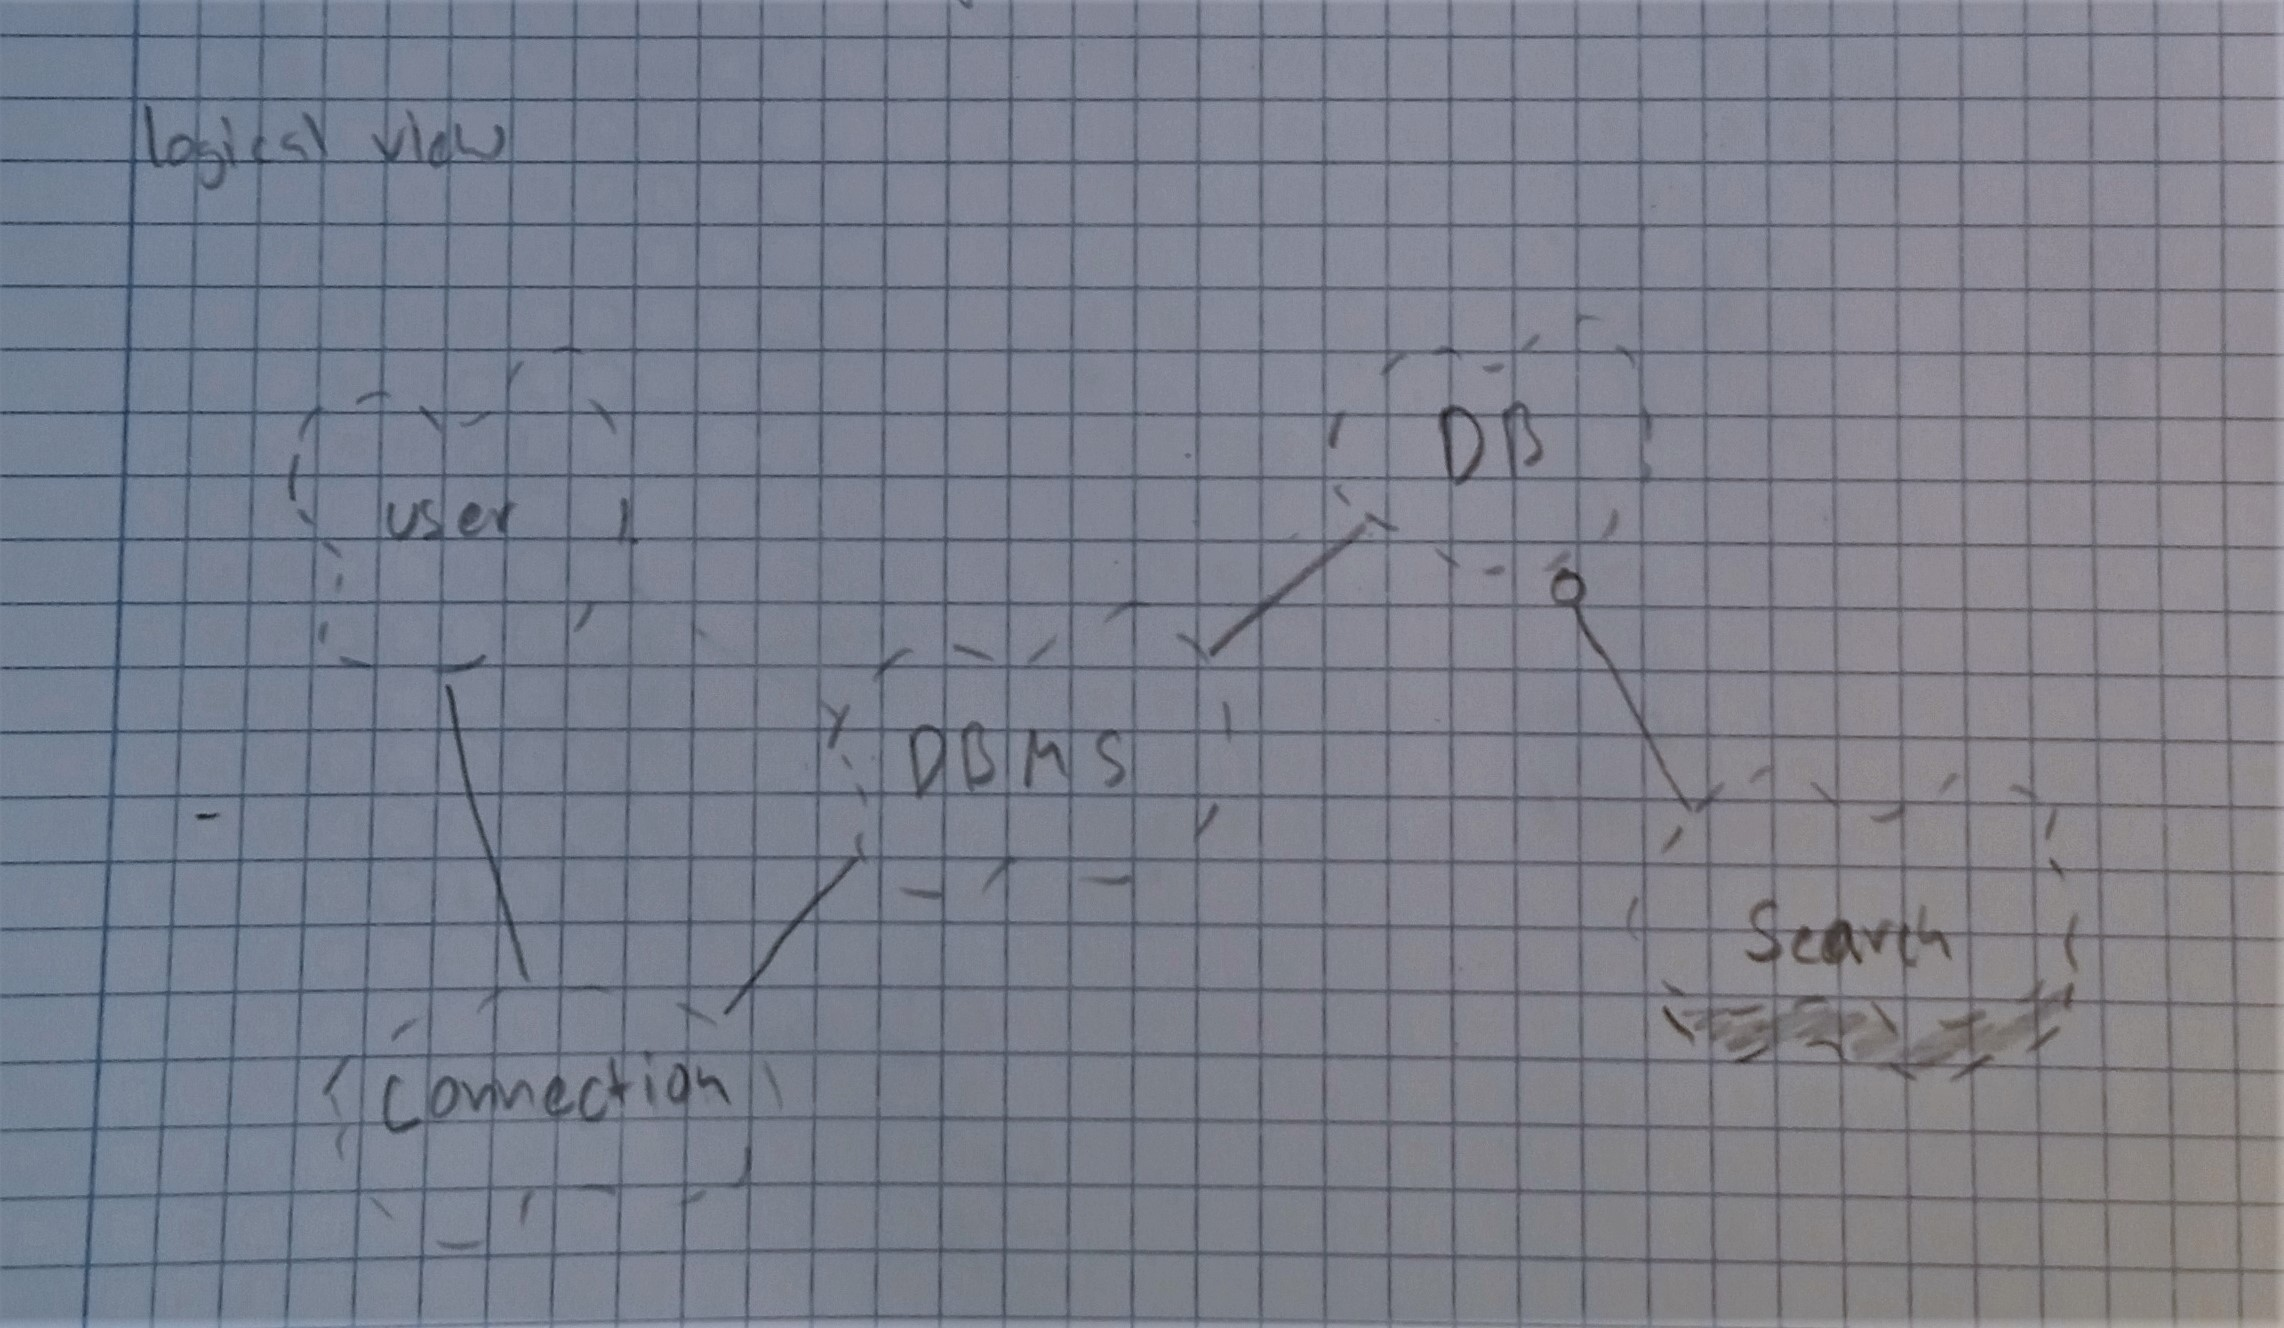
\includegraphics[width=\textwidth]{Immagini/IMG_20230604_17asdfg1749.jpg}
  \caption{Logical View}
\end{figure}


\begin{figure}[hbt]
\section{Implementation View}
  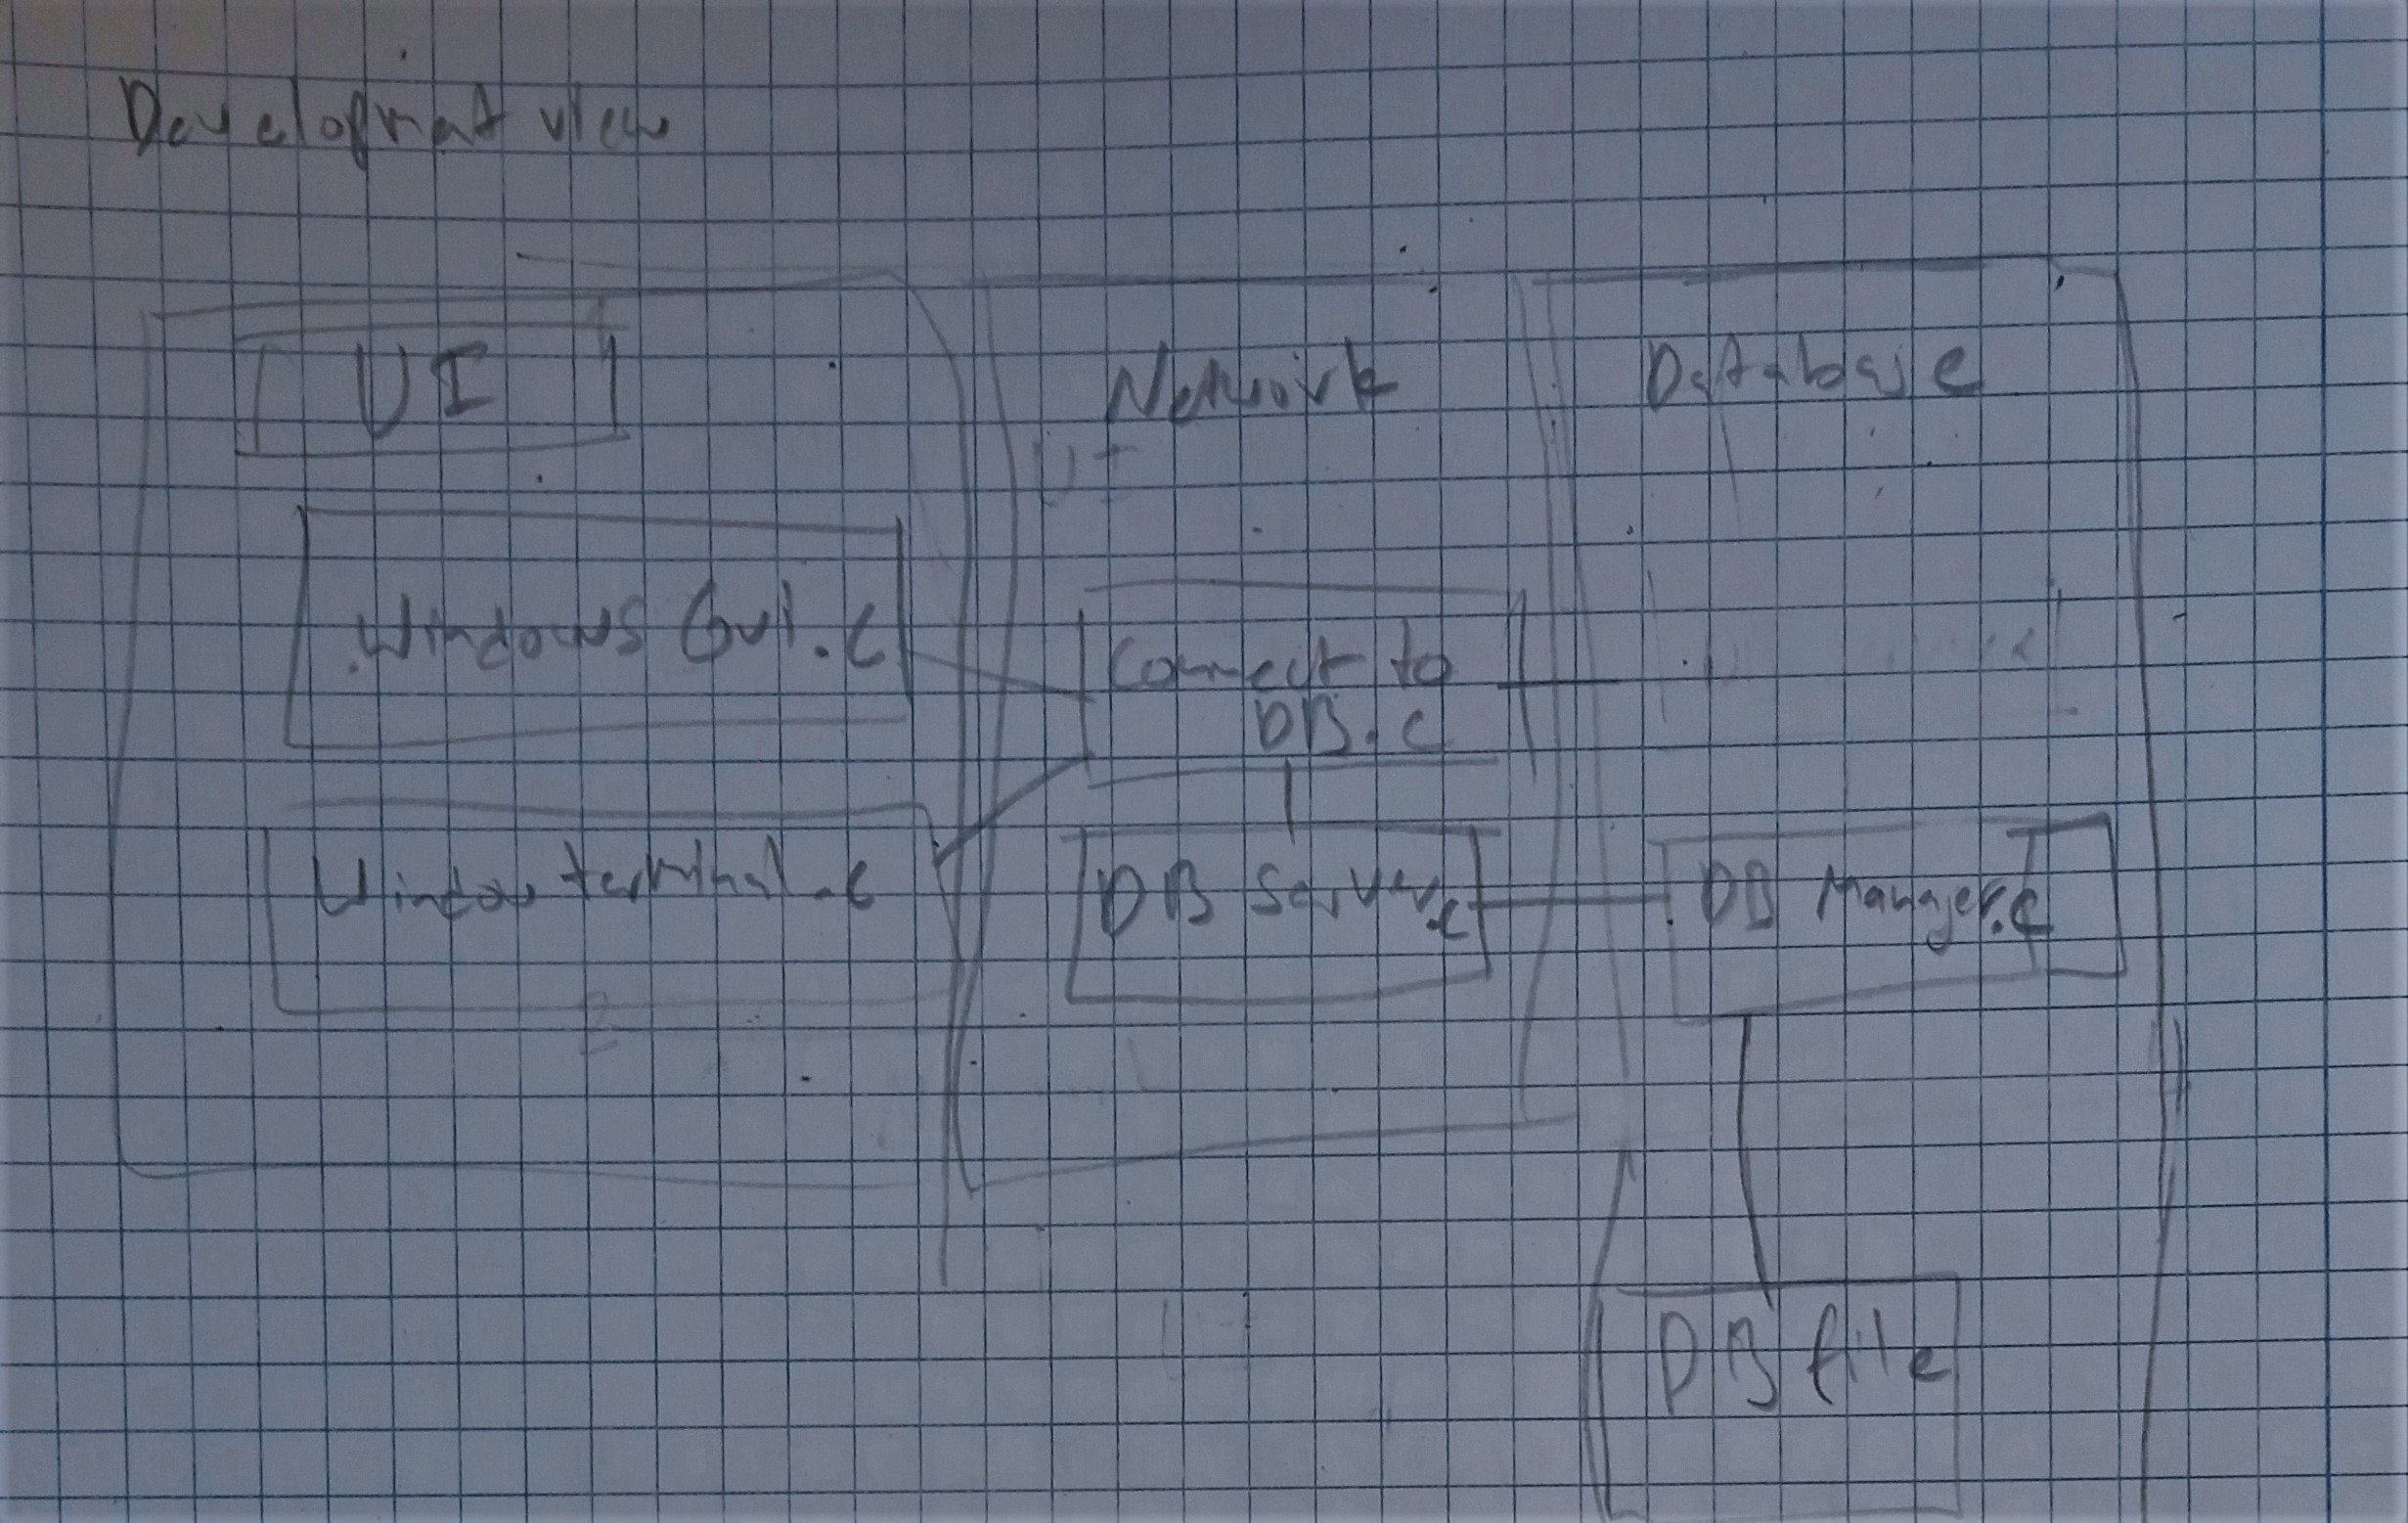
\includegraphics[width=\textwidth]{Immagini/IMG_20230604_171802.jpg}
  \caption{Implementation View}
\end{figure}

\begin{figure}[hbt]
\section{Process View}
GUI event handler ensures that the user can press the buttons without having to wait for the connection to be completed. DB client establishes the connection, waits for the server. DB webserver connects and sends information to DB client and talks to B manager. DB manager processes data and searches data while server does other things.

  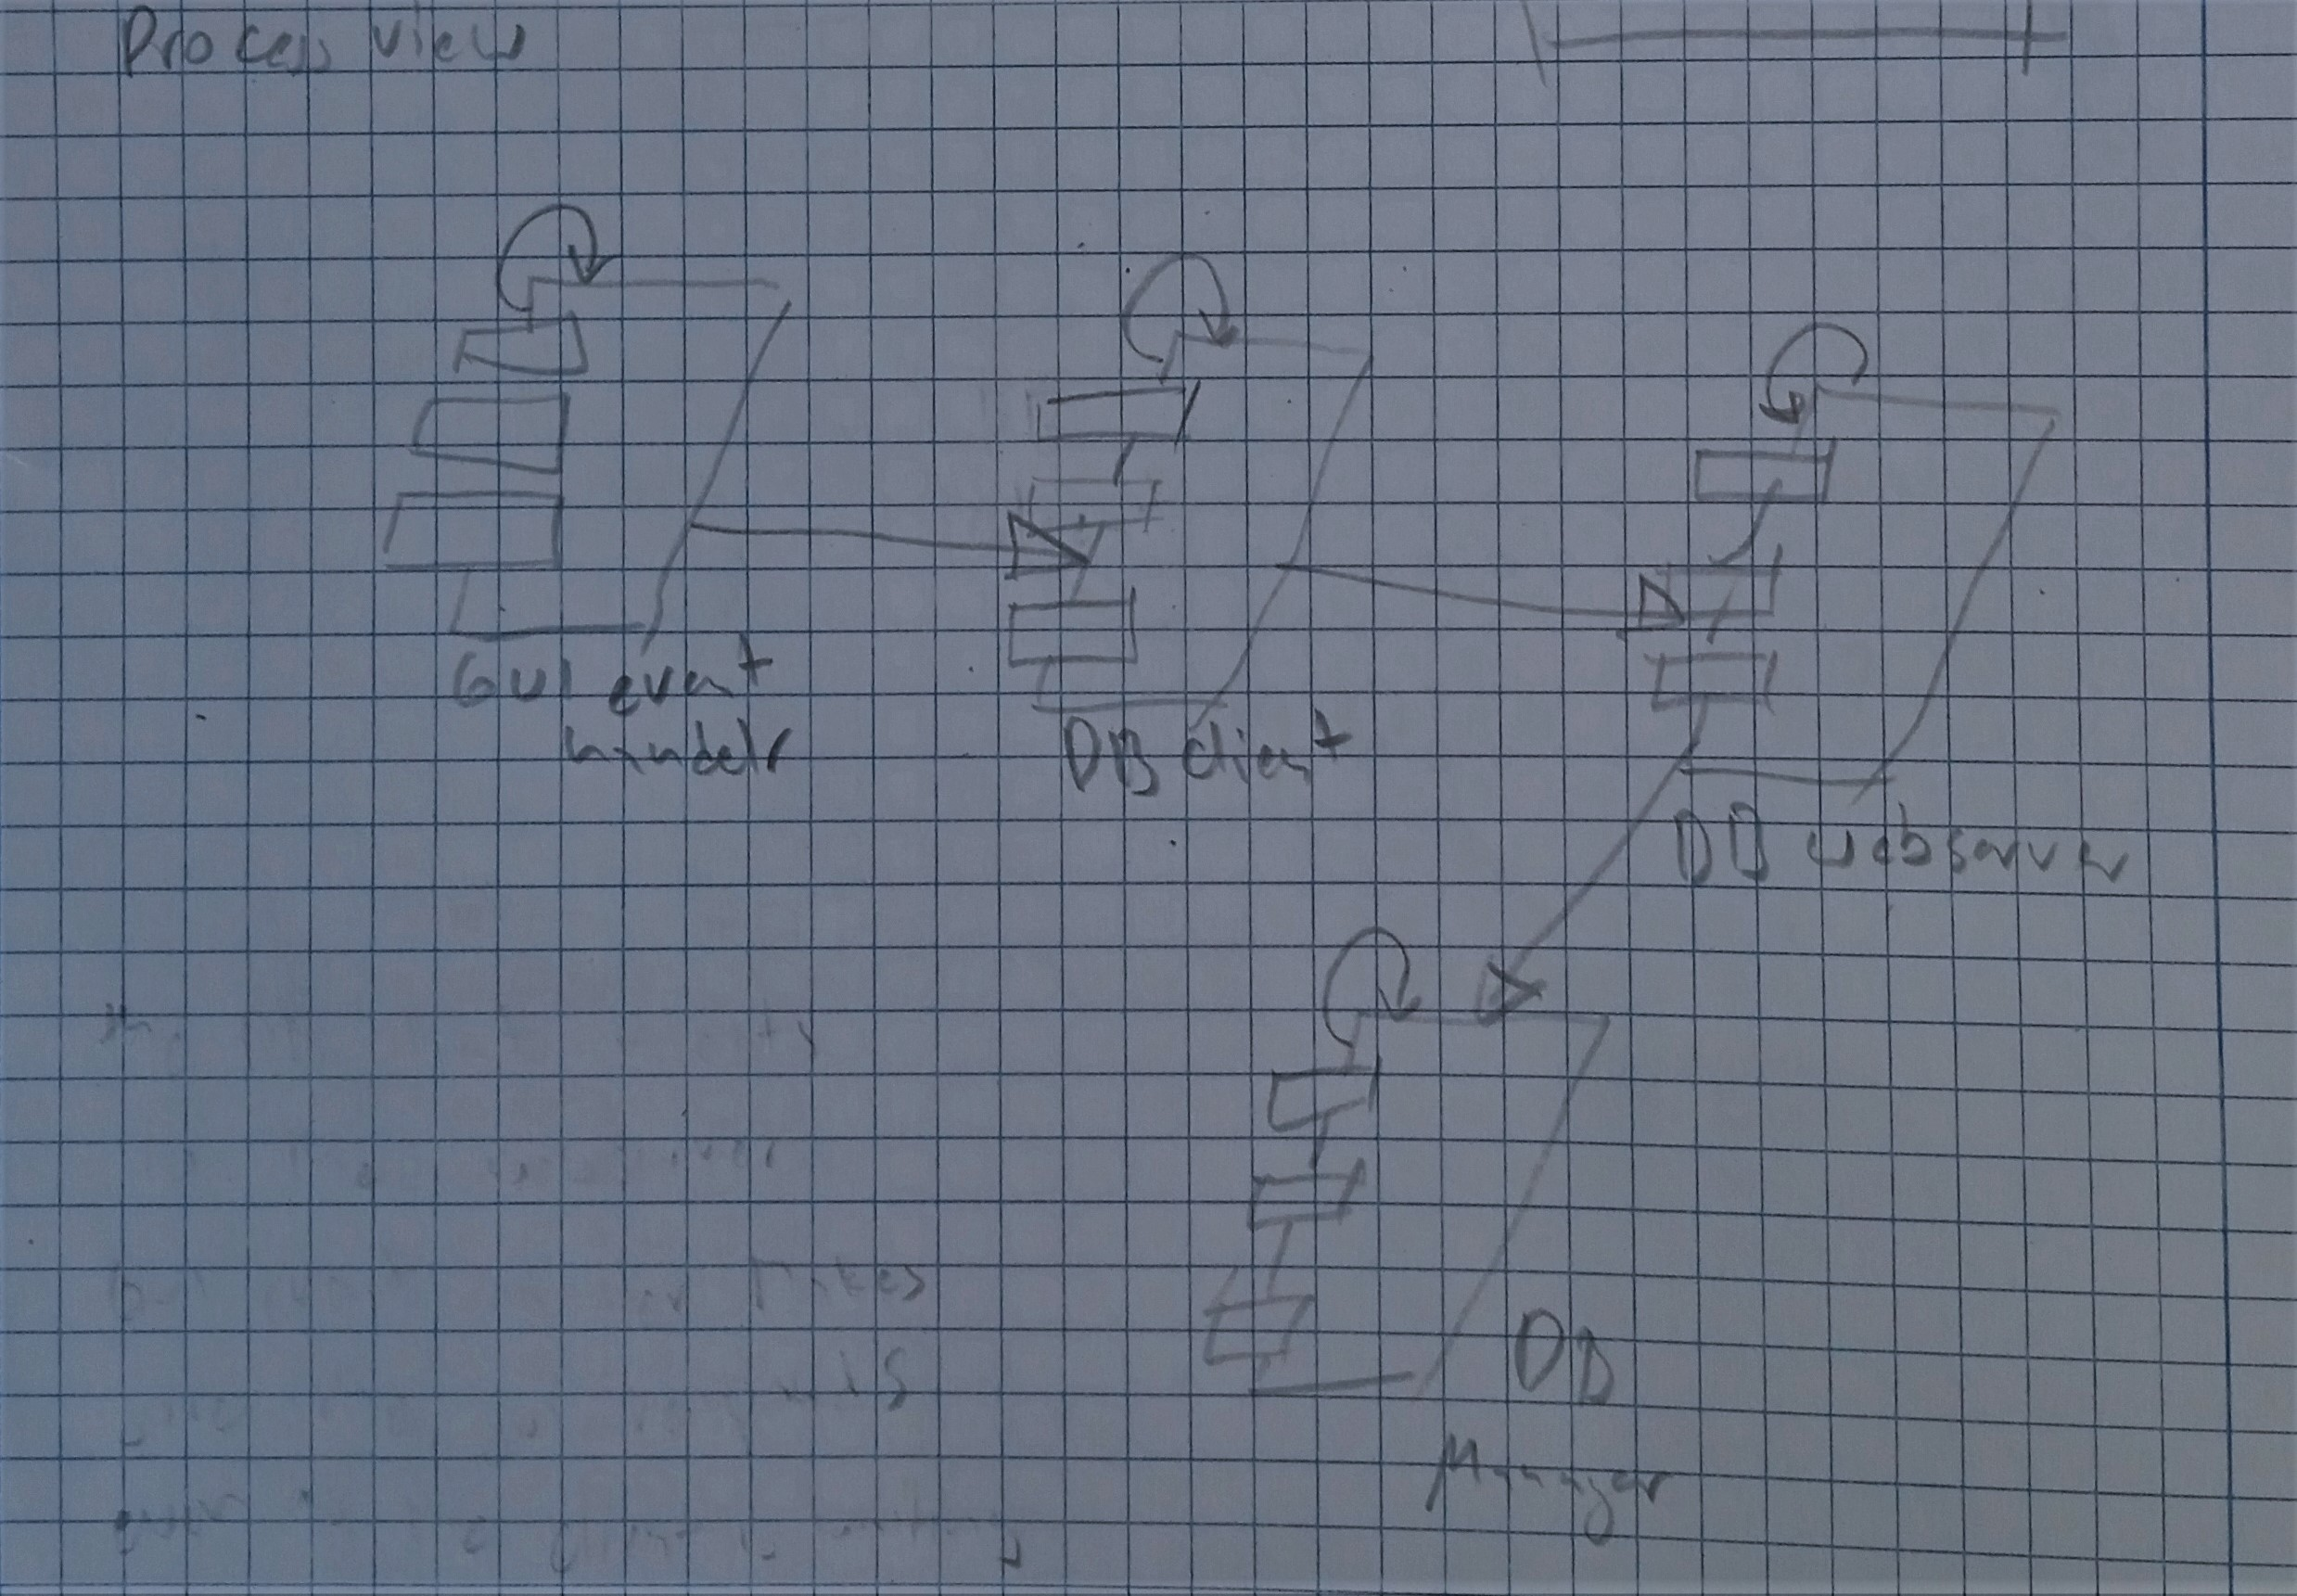
\includegraphics[width=\textwidth]{Immagini/IMG_20230604dhjj_171802.jpg}
  \caption{Process View}
\end{figure}

\begin{figure}[hbt]
\section{Distribution View}
  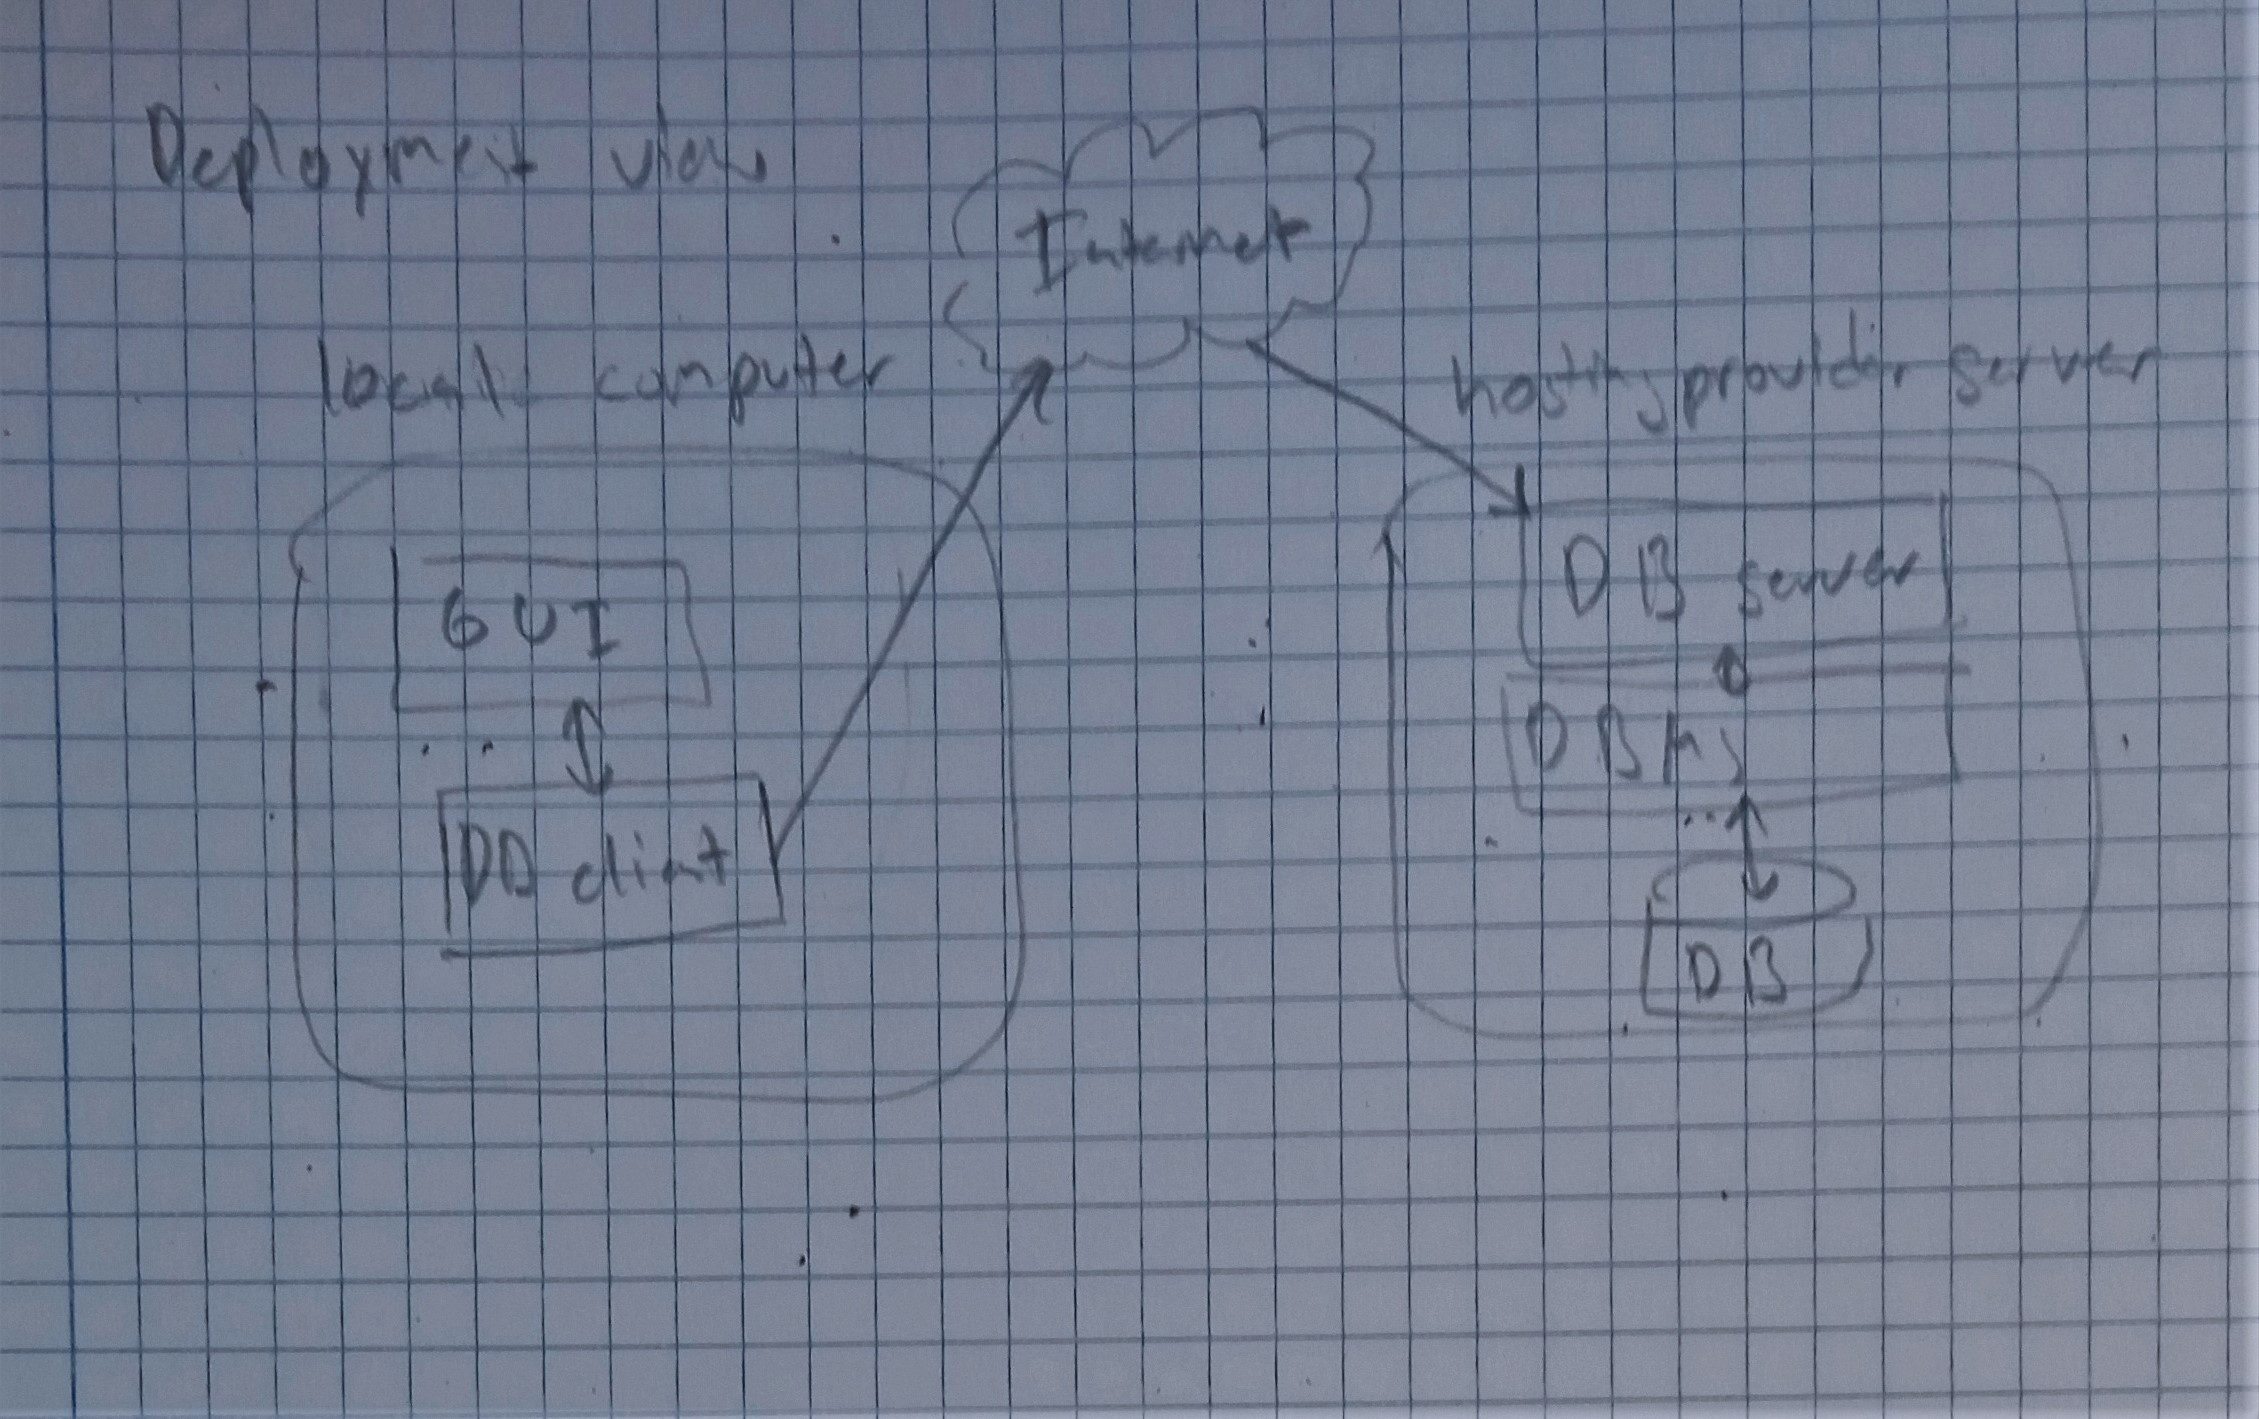
\includegraphics[width=\textwidth]{Immagini/IMG_20230604_171821.jpg}
  \caption{Distribution View}
\end{figure}
